
\documentclass{beamer}
\usecolortheme{dove}
\setbeamertemplate{navigation symbols}{}
\usepackage{amsmath,amssymb,amsfonts,amsthm, multicol, subfigure, color}
\usepackage{bm}
\usepackage{graphicx}
\usepackage{tabularx}
\usepackage{booktabs}
\usepackage{hyperref}
\usepackage{pdfpages}
\usepackage{xcolor}
\definecolor{seagreen}{RGB}{46, 139, 87}
\definecolor{mustard}{RGB}{234, 170, 0}
\def\independenT#1#2{\mathrel{\rlap{$#1#2$}\mkern2mu{#1#2}}}
\newcommand\indep{\protect\mathpalette{\protect\independenT}{\perp}}
\def\log{\text{log}}
\newcommand\logit{\text{logit}}
\newcommand\iid{\stackrel{\text{iid}}{\sim}}
\newcommand\E{\text{E}}
\newcommand\V{\text{V}}
\renewcommand\P{\text{P}}
\newcommand{\Cov}{\text{Cov}}
\newcommand{\Cor}{\text{Cor}}
\newcommand\doop{\texttt{do}}
\usepackage{stackrel}
\usepackage{tikz}
\usetikzlibrary{arrows,shapes.arrows,positioning,shapes,patterns,calc}
\newcommand\slideref[1]{\vskip .1cm \tiny \textcolor{gray}{{#1}}}
\newcommand\red[1]{\color{red}#1}
\newcommand\blue[1]{\color{blue}#1}
\newcommand\gray[1]{\color{gray}#1}
\newcommand\seagreen[1]{\color{seagreen}#1}
\newcommand\purple[1]{\color{purple}#1}
\newcommand\orange[1]{\color{orange}#1}
\newcommand\black[1]{\color{black}#1}
\newcommand\white[1]{\color{white}#1}
\newcommand\teal[1]{\color{teal}#1}
\newcommand\magenta[1]{\color{magenta}#1}
\newcommand\Fuchsia[1]{\color{Fuchsia}#1}
\newcommand\BlueGreen[1]{\color{BlueGreen}#1}
\newcommand\bblue[1]{\textcolor{blue}{\textbf{#1}}}
\newcommand\bred[1]{\textcolor{red}{\textbf{#1}}}
\newcommand\bgray[1]{\textcolor{gray}{\textbf{#1}}}
\newcommand\bgreen[1]{\textcolor{seagreen}{\textbf{#1}}}
\newcommand\bref[2]{\href{#1}{\color{blue}{#2}}}
\colorlet{lightgray}{gray!40}
\pgfdeclarelayer{bg}    % declare background layer for tikz
\pgfsetlayers{bg,main} % order layers for tikz
\newcommand\mycite[1]{\begin{scriptsize}\textcolor{darkgray}{(#1)}\end{scriptsize}}
\newcommand{\tcframe}{\frame{
%\small{
\only<1|handout:0>{\tableofcontents}
\only<2|handout:1>{\tableofcontents[currentsubsection]}}
%}
}

\newcommand{\goalsframe}{\begin{frame}{Learning goals for today}
By the end of class, you will be able to
\begin{itemize}
\item articulate a clear research question
\item use language appropriate for causal or descriptive questions
\end{itemize} \vskip .2in
\end{frame}}

\usepackage[round]{natbib}
\bibliographystyle{humannat-mod}
\setbeamertemplate{enumerate items}[default]
\usepackage{mathtools}

\title{Studying Social Inequality with Data Science}
\author{Ian Lundberg}
\date{\today}

\begin{document}

\begin{frame}
\begin{tikzpicture}[x = \textwidth, y = \textheight]
\node at (0,0) {};
\node at (1,1) {};
\node[anchor = north west, align = left, font = \huge] at (0,.9) {Studying\\Social Inequality\\with Data Science};
\node[anchor = north east, align = right] (number) at (1,.9) {INFO 3370 / 5371\\Spring 2023};
\node[anchor = north, font = \Large, align = left] at (.5,.5) {\bblue{Asking Research Questions}};
\end{tikzpicture}
\end{frame}

\goalsframe

\begin{frame}
What makes a good research question?
\end{frame}

%\begin{frame}
%\includegraphics[height = .8\textheight]{estimands_title} \hfill \bref{https://doi.org/10.1177/00031224211004187}{[link]}
%\end{frame}

\begin{frame}{Keys to a good research question} \pause
\begin{enumerate}
\item a unit of analysis
\begin{itemize}
\item a row of your dataset \pause
\end{itemize}
\item an outcome
\begin{itemize}
\item a variable with a value for each unit \pause
\end{itemize}
\item a target population
\begin{itemize}
\item a set of units about whom to infer
\item clear who is included and who is not
\end{itemize} \pause
\item potential for surprising results
\end{enumerate}
\end{frame}

% DESCRIBE POPULATION
\begin{frame}[t]
\begin{tikzpicture}[x = \textwidth, y = .8\textheight]
\node at (0,0) {};
\node at (1,1) {};
\node[anchor = west, font = {\large\bf}] (goal) at (0, .9) {Describe a population};
\draw[line width = 1.5pt, line cap = round] (goal.south west) -- (goal.south east);
\node[anchor = west] at (0, .75) {What is the proportion employed};
\node[anchor = west] at (0, .68) {among U.S. resident women ages 21--35?};
% Title rows
\only<2->{
\node[font = \footnotesize, anchor = east] at (.4, .4) {Woman 1};
\node[font = \footnotesize, anchor = east] at (.4, .35) {Woman 2};
\node[font = \footnotesize, anchor = east] at (.4, .3) {Woman 3};
\node[font = \footnotesize, anchor = east] at (.4, .25) {Woman 4};
}
\only<3->{
% Title columns
\node[font = \footnotesize, anchor = south] (emp) at (.5, .45) {Employed?};
\draw[thick] (.4,.45) -- (.6, .45);
% Cell values
\node[font = \footnotesize] at (.5, .4) {1};
\node[font = \footnotesize] at (.5, .35) {0};
\node[font = \footnotesize] at (.5, .3) {1};
\node[font = \footnotesize] at (.5, .25) {1};
}
\end{tikzpicture}
\end{frame}

% DESCRIBE POPULATION SUBGROUPS
\begin{frame}[t]
\begin{tikzpicture}[x = \textwidth, y = .8\textheight]
\node at (0,0) {};
\node at (1,1) {};
\node[anchor = west, font = {\large\bf}] (goal) at (0, .9) {Describe population subgroups};
\draw[line width = 1.5pt, line cap = round] (goal.south west) -- (goal.south east);
\node[anchor = west] at (0, .75) {What is the proportion employed};
\node[anchor = west] at (0, .68) {among U.S. resident women ages 21--35,};
\node[anchor = west] at (0, .61) {comparing mothers to non-mothers?};
% MOTHERS
% Title rows
\only<2->{
\node[font = \footnotesize, anchor = east] at (.2, .4) {Mother 1};
\node[font = \footnotesize, anchor = east] at (.2, .35) {Mother 2};
\node[font = \footnotesize, anchor = east] at (.2, .3) {Mother 3};
\node[font = \footnotesize, anchor = east] at (.2, .25) {Mother 4};
% Title columns
\node[font = \footnotesize, anchor = south] (emp) at (.3, .45) {Employed?};
\draw[thick] (.2,.45) -- (.4, .45);
% Cell values
\node[font = \footnotesize] at (.3, .4) {0};
\node[font = \footnotesize] at (.3, .35) {0};
\node[font = \footnotesize] at (.3, .3) {0};
\node[font = \footnotesize] at (.3, .25) {1};
% NON-MOTHERS
% Title rows
\node[font = \footnotesize, anchor = east] at (.7, .4) {Non-Mother 1};
\node[font = \footnotesize, anchor = east] at (.7, .35) {Non-Mother 2};
\node[font = \footnotesize, anchor = east] at (.7, .3) {Non-Mother 3};
\node[font = \footnotesize, anchor = east] at (.7, .25) {Non-Mother 4};
% Title columns
\node[font = \footnotesize, anchor = south] (emp) at (.8, .45) {Employed?};
\draw[thick] (.7,.45) -- (.9, .45);
% Cell values
\node[font = \footnotesize] at (.8, .4) {1};
\node[font = \footnotesize] at (.8, .35) {0};
\node[font = \footnotesize] at (.8, .3) {1};
\node[font = \footnotesize] at (.8, .25) {1};
}
\end{tikzpicture}
\end{frame}

% CAUSAL EFFECT IN A POPULATION
\begin{frame}[t]
\begin{tikzpicture}[x = \textwidth, y = .8\textheight]
\node at (0,0) {};
\node at (1,1) {};
\node[anchor = west, font = {\large\bf}] (goal) at (0, .9) {Causal effect in a population};
\draw[line width = 1.5pt, line cap = round] (goal.south west) -- (goal.south east);
\node[anchor = west] at (0, .75) {What is the causal effect of motherhood on employment};
\node[anchor = west] at (0, .68) {among U.S. resident women ages 21--35?};
\only<2->{
% Title rows
\node[font = \footnotesize, anchor = east] at (.2, .3) {Woman 1};
\node[font = \footnotesize, anchor = east] at (.2, .25) {Woman 2};
\node[font = \footnotesize, anchor = east] at (.2, .2) {Woman 3};
\node[font = \footnotesize, anchor = east] at (.2, .15) {Woman 4};
}
\only<3->{
% Title column 1
\node[font = \footnotesize, anchor = south, align = center] (emp) at (.3, .35) {Would be\\employed if\\a mother?\\$Y(1)$};
\draw[thick] (.22,.35) -- (.38, .35);
% Cell values 1
\node[font = \footnotesize] at (.3, .3) {0};
\node[font = \footnotesize] at (.3, .25) {0};
\node[font = \footnotesize] at (.3, .2) {0};
\node[font = \footnotesize] at (.3, .15) {1};
}
\only<4->{
% Title column 0
\node[font = \footnotesize, anchor = south, align = center] (emp) at (.5, .35) {Would be\\employed if\\a non-mother?\\$Y(0)$};
\draw[thick] (.42,.35) -- (.58, .35);
% Cell values 0
\node[font = \footnotesize] at (.5, .3) {1};
\node[font = \footnotesize] at (.5, .25) {0};
\node[font = \footnotesize] at (.5, .2) {1};
\node[font = \footnotesize] at (.5, .15) {1};
}
\only<5->{
% Title column causal
\node[font = \footnotesize, anchor = south, align = center] (emp) at (.7, .35) {Causal\\effect\\$Y(1) - Y(0)$};
\draw[thick] (.62,.35) -- (.78, .35);
% Cell values causal
\node[font = \footnotesize] at (.7, .3) {-1};
\node[font = \footnotesize] at (.7, .25) {0};
\node[font = \footnotesize] at (.7, .2) {-1};
\node[font = \footnotesize] at (.7, .15) {0};
}
\end{tikzpicture}
\end{frame}

% CONTRAST THOSE TWO
\begin{frame}[t]
\begin{tikzpicture}[x = \textwidth, y = .8\textheight]
\node at (0,0) {};
\node at (1,1) {};
\node[anchor = west] at (0,.75) {\scalebox{.5}{
\begin{tikzpicture}[x = \textwidth, y = .8\textheight]
\node at (0,0) {};
\node at (1,1) {};
\node[anchor = west, font = {\large\bf}] (goal) at (0, .9) {Describe population subgroups};
\draw[line width = 1.5pt, line cap = round] (goal.south west) -- (goal.south east);
\node[anchor = west] at (0, .75) {What is the proportion employed};
\node[anchor = west] at (0, .68) {among U.S. resident women ages 21--35,};
\node[anchor = west] at (0, .61) {comparing mothers to non-mothers?};
% MOTHERS
% Title rows
\node[font = \footnotesize, anchor = east] at (.2, .4) {Mother 1};
\node[font = \footnotesize, anchor = east] at (.2, .35) {Mother 2};
\node[font = \footnotesize, anchor = east] at (.2, .3) {Mother 3};
\node[font = \footnotesize, anchor = east] at (.2, .25) {Mother 4};
% Title columns
\node[font = \footnotesize, anchor = south] (emp) at (.3, .45) {Employed?};
\draw[thick] (.2,.45) -- (.4, .45);
% Cell values
\node[font = \footnotesize] at (.3, .4) {0};
\node[font = \footnotesize] at (.3, .35) {0};
\node[font = \footnotesize] at (.3, .3) {0};
\node[font = \footnotesize] at (.3, .25) {1};
% NON-MOTHERS
% Title rows
\node[font = \footnotesize, anchor = east] at (.7, .4) {Non-Mother 1};
\node[font = \footnotesize, anchor = east] at (.7, .35) {Non-Mother 2};
\node[font = \footnotesize, anchor = east] at (.7, .3) {Non-Mother 3};
\node[font = \footnotesize, anchor = east] at (.7, .25) {Non-Mother 4};
% Title columns
\node[font = \footnotesize, anchor = south] (emp) at (.8, .45) {Employed?};
\draw[thick] (.7,.45) -- (.9, .45);
% Cell values
\node[font = \footnotesize] at (.8, .4) {1};
\node[font = \footnotesize] at (.8, .35) {0};
\node[font = \footnotesize] at (.8, .3) {1};
\node[font = \footnotesize] at (.8, .25) {1};
\end{tikzpicture}
}};
\node[anchor = west] at (0,.25) {\scalebox{.5}{
\begin{tikzpicture}[x = \textwidth, y = .8\textheight]
\node at (0,0) {};
\node at (1,1) {};
\node[anchor = west, font = {\large\bf}] (goal) at (0, .9) {Causal effect in a population};
\draw[line width = 1.5pt, line cap = round] (goal.south west) -- (goal.south east);
\node[anchor = west] at (0, .75) {What is the causal effect of motherhood on employment};
\node[anchor = west] at (0, .68) {among U.S. resident women ages 21--35?};
% Title rows
\node[font = \footnotesize, anchor = east] at (.2, .3) {Woman 1};
\node[font = \footnotesize, anchor = east] at (.2, .25) {Woman 2};
\node[font = \footnotesize, anchor = east] at (.2, .2) {Woman 3};
\node[font = \footnotesize, anchor = east] at (.2, .15) {Woman 4};
% Title columns
\node[font = \footnotesize, anchor = south, align = center] (emp) at (.3, .35) {Would be\\employed if\\a mother?\\$Y(1)$};
\node[font = \footnotesize, anchor = south, align = center] (emp) at (.5, .35) {Would be\\employed if\\a non-mother?\\$Y(0)$};
\node[font = \footnotesize, anchor = south, align = center] (emp) at (.7, .35) {Causal\\effect\\$Y(1) - Y(0)$};
\draw[thick] (.22,.35) -- (.38, .35);
\draw[thick] (.42,.35) -- (.58, .35);
\draw[thick] (.62,.35) -- (.78, .35);
% Cell values
\node[font = \footnotesize] at (.3, .3) {0};
\node[font = \footnotesize] at (.3, .25) {0};
\node[font = \footnotesize] at (.3, .2) {0};
\node[font = \footnotesize] at (.3, .15) {1};
\node[font = \footnotesize] at (.5, .3) {1};
\node[font = \footnotesize] at (.5, .25) {0};
\node[font = \footnotesize] at (.5, .2) {1};
\node[font = \footnotesize] at (.5, .15) {1};
\node[font = \footnotesize] at (.7, .3) {-1};
\node[font = \footnotesize] at (.7, .25) {0};
\node[font = \footnotesize] at (.7, .2) {-1};
\node[font = \footnotesize] at (.7, .15) {0};
\end{tikzpicture}
}};
\node[align = center, font = \large] at (.85,.5) {Very\\\bblue{different}\\research\\goals};
\draw[->, thick] (.75, .6) -- (.68,.68);
\draw[->, thick] (.75, .4) -- (.68,.32);
%\draw[->, thick] (.75, .65) to[out = 110, in = 0] (.63,.75);
%\draw[->, thick] (.75, .35) to[out = 250, in = 0] (.63,.25);
\end{tikzpicture}
\end{frame}

\begin{frame}{Keywords: What kind of question is being asked?}
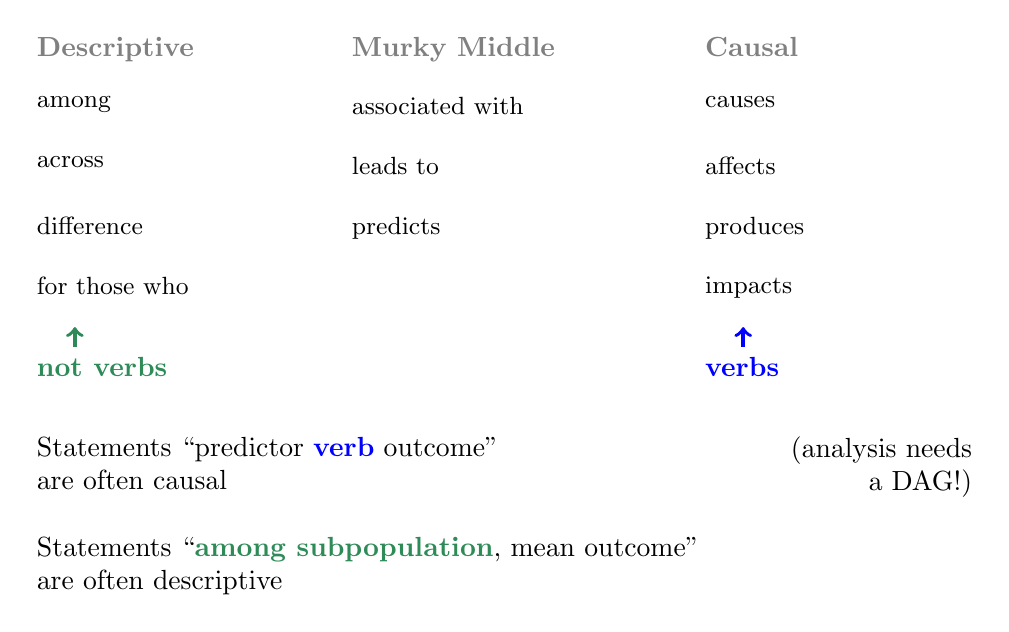
\begin{tikzpicture}[x = \textwidth, y = 1in] \pause
\node[anchor = north west, font = \bf, gray] at (0,0) {Descriptive};
\node[anchor = north west, font = \small] at (0,-.3) {among};
\node[anchor = north west, font = \small] at (0,-.6) {across};
\node[anchor = north west, font = \small] at (0,-.9) {difference};
\node[anchor = north west, font = \small] at (0,-1.2) {for those who}; \pause
\node[anchor = north west, font = \bf, gray] at (.7,0) {Causal};
\node[anchor = north west, font = \small] at (.7,-.3) {causes};
\node[anchor = north west, font = \small] at (.7,-.6) {affects};
\node[anchor = north west, font = \small] at (.7,-.9) {produces};
\node[anchor = north west, font = \small] at (.7,-1.2) {impacts}; \pause
\node[anchor = north west, font = \bf, gray] at (.33,0) {Murky Middle};
\node[anchor = north west, font = \small] at (.33,-.3) {associated with};
\node[anchor = north west, font = \small] at (.33,-.6) {leads to};
\node[anchor = north west, font = \small] at (.33,-.9) {predicts}; \pause
\node[anchor = north west, font = \bf, blue] at (.7,-1.6) {verbs};
\draw[->, line width = 1.3pt, blue] (.75,-1.6) -- (.75,-1.5); \pause
\node[anchor = north west, font = \bf, seagreen] at (0,-1.6) {not verbs};
\draw[->, line width = 1.3pt, seagreen] (.05,-1.6) -- (.05,-1.5); \pause
\node[anchor = north west, align = left] at (0,-2) {Statements ``predictor \bblue{verb} outcome''\\are often causal}; 
\node[anchor = north east, align = right] at (1,-2) {(analysis needs\\a DAG!)}; \pause
\node[anchor = north west, align = left] at (0,-2.5) {Statements ``\bgreen{among subpopulation}, mean outcome''\\are often descriptive};
\end{tikzpicture}
\end{frame}

\begin{frame}

A good project may have a very simple question

\end{frame}

\begin{frame}{Example: Prevalence of housing eviction}{Lundberg \& Donnelly \bref{https://doi.org/10.1007/s13524-018-0735-y}{2019}}

What proportion of children born in large U.S. cities in 1998--2000\\
was ever evicted from their home from birth to age 15? \vskip .1in

\begin{itemize}
\item<2-> unit of analysis
\begin{itemize}
\item<3-> a child
\end{itemize}
\item<2-> target population
\begin{itemize}
\item<4-> children born in large U.S. cities in 1998--2000
\item<5-> (and subgroups by race and income)
\end{itemize}
\item<2-> outcome
\begin{itemize}
\item<6-> evicted from home between birth and age 15
\end{itemize}
\end{itemize}

\end{frame}


\begin{frame}{Example: Prevalence of housing eviction}{Lundberg \& Donnelly \bref{https://doi.org/10.1007/s13524-018-0735-y}{2019}}
\centering
\href{https://ffcws.princeton.edu/}{\includegraphics[width = \textwidth]{ffcws}} \pause \vskip .2in
\includegraphics[width = \textwidth, trim = 0 4.3in 0 0, clip]{ffcws_question}\\ \pause
\includegraphics[width = \textwidth, trim = 0 2.7in 0 2.2in, clip]{ffcws_question}\\
\includegraphics[width = \textwidth, trim = 0 0 0 4.9in, clip]{ffcws_question} \vskip .2in \pause
\begin{itemize}
\item we filled in missing values with regression \pause
\item we gathered responses across years
\end{itemize}

\end{frame}

\begin{frame}{Example: Prevalence of housing eviction}{Lundberg \& Donnelly \bref{https://doi.org/10.1007/s13524-018-0735-y}{2019}}
\centering
\includegraphics[width = .8\textwidth]{eviction_result}
\end{frame}

\begin{frame}{Example: Progress toward gender equality}{From Homework 2: England, Levine, \& Mishel \bref{https://doi.org/10.1073/pnas.1918891117}{2020}}
\centering
\includegraphics<2>[width = .9\textwidth]{gender_emp}
\includegraphics<3>[width = .9\textwidth]{gender_wage}
\end{frame}

\begin{frame}

hypothetical examples of questions

\end{frame}

\begin{frame}{Example: Not right for our class} \pause

Researcher uses a random forest \pause
\begin{itemize}
\item models hourly wage given many inputs \pause
\item reports a measure of variable importance
\begin{itemize}
\item how important is each variable in predicting wage? 
\end{itemize}
\end{itemize} \pause \vskip .2in
Why is this question not suitable for our class project? \pause
\begin{itemize}
\item we want a study of the world,\\and this is more a study of an algorithm \pause
\item we want a clear target population,\\and there isn't one here \pause
\item we want an outcome aggregated within subgroups,\\and this is something else
\end{itemize}

\end{frame}

\begin{frame}{Example: Could be improved (1 / 3)}

A researcher studies the racial composition of those
\begin{itemize}
\item with college degrees
\item without college degrees
\end{itemize}
among 25--50 year old American residents in 2022 \pause \vskip .2in

What is your biggest concern about this study? \pause
\begin{itemize}
\item usually it is best of $X$ precedes $Y$ \pause
\item better to study $\P(\text{College} \mid \text{Race})$\\instead of $\P(\text{Race}\mid\text{College})$
\end{itemize}

\end{frame}

\begin{frame}{Example: Could be improved (2 / 3)}

A researcher studies whether those with higher hourly wages\\have higher annual earnings \vskip .3in
What is your biggest concern about this study? \pause
\begin{itemize}
\item needs a clearer target population \pause
\item result is somewhat obvious:\\hard to argue that those with higher hourly wages\\would have lower annual earnings
\end{itemize}

\end{frame}

\begin{frame}{Example: Could be improved (3 / 3)}

A researcher uses a probability sample survey to estimate the share of total wealth held by the top 1\% of households \pause
\begin{itemize}
\item 30\% of sampled individuals refuse to answer \pause
\item the researcher drops them \pause
\item they say the target population is the top 1\% wealth share among households willing to respond to the survey
\end{itemize} \vskip .3in \pause
What is your biggest concern about this study? \pause
\begin{itemize}
\item the target population is not very interesting\\if it excludes those who won't respond
\end{itemize}

\end{frame}

\begin{frame}{Keys to a good research question}
\begin{enumerate}
\item a unit of analysis
\begin{itemize}
\item a row of your dataset
\end{itemize}
\item an outcome
\begin{itemize}
\item a variable with a value for each unit
\end{itemize}
\item a target population
\begin{itemize}
\item a set of units about whom to infer
\item clear who is included and who is not
\end{itemize}
\end{enumerate}
\end{frame}

\goalsframe

\end{document}

